%!TEX root = ../report.tex

\chapter{Methodology}

This chapter and the equations mentioned here were adapted from the survey on Active Learning \cite{Settles2010}.

\section{Active Learning}
Active learning belongs to a special case of semi-supervised learning algorithm where the learner is allowed to query the user to get the labels for data points which will help the learner to perform better \cite{active_learning}\cite{Settles2010}. According to \cite{Settles2010}, when the learner is allowed to choose the data points for learning,  the performance of the learner is better with less labeled data.   

Supervised learning algorithm performs well when the model is trained with a large number of labeled instances. But the labeled instances are expensive, time-consuming, and difficult to obtain.  Active learning helps in overcoming the situations where there is plenty of unlabeled data is available which are difficult to label or the cost of labeling them is high. The main aim of the active learning is to improve the accuracy by labeling less number of instances. The instances that need to be labeled is determined by the active learning query strategies.\cite{Settles2010}

\begin{figure}[h!]
	\centering
	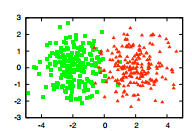
\includegraphics[scale=1]{images/sample_data}
	\caption{Sample data points  in a 2D feature space . Image from \cite{Settles2010}.}
	\label{sample_data}
\end{figure}

Let us consider the Fig \ref{sample_data} based on experiments done by \cite{Settles2010}. It consists of 400 2-dimensional data points from two Gaussian centered  (-2,0) and (2,0) having standard deviation $\sigma$ = 1.  These data points belong to two classes. (each class has 200 data points).

\begin{figure}[h!]
	\centering
	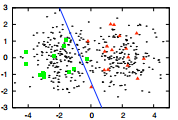
\includegraphics[scale=1]{images/random_sampling}
	\caption{Decision boundary obtained by random sampling. Image from \cite{Settles2010}.}
	\label{random_sampling}
\end{figure}

Fig \ref{random_sampling} shows the decision boundary obtained using a supervised learning approach after selecting 30 data points randomly for labeling. We can infer from the line that the linear decision boundary fitted by a logistic regression model is sub-optimal. This model achieves 70 \% accuracy on the remaining unlabeled points because of the poor selection of data points for labeling.

\begin{figure}[h!]
	\centering
	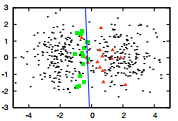
\includegraphics[scale=1]{images/active_sampling}
	\caption{Decision boundary obtained by sampling using active learnig strategies. Image from \cite{Settles2010}.}
	\label{active_sampling}
\end{figure}


Fig \ref{active_sampling} shows the decision boundary obtained using active learning approach. The active learning approach selects 30 points close to the decision boundary for labeling. By using the label for these data points, the classifier achieves 90 \% accuracy which is significantly better than the approach by random sampling of data points. \cite{Settles2010}

\section{Active Learning Scenarios}

There are three main problem scenario that can occur when the learner queries the user. They are 
\begin{itemize}
	\item membership query synthesis
	\item stream-based selective sampling
	\item pool-based sampling
\end{itemize}

\subsection{Membership query synthesis}
In membership query synthesis, the learner is allowed to choose any unlabeled data points which can include the a new query that the learner generates from the underlying distribution instead of the existing data points. \\
\begin{figure}[h!]
	\centering
	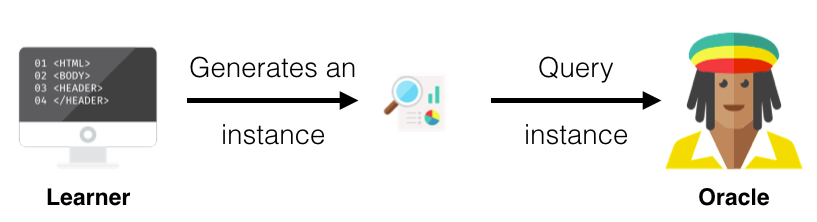
\includegraphics[scale=0.4]{images/membership}
	\caption{Membership query synthesis. Image from \cite{active_learning_datacamp}.}
	\label{membership}
\end{figure}\\
Fig \ref{membership} shows the workflow of membership query synthesis.The shortcoming of this setting is that the query generated by the learner can sometimes be unrecognized for the human to label. When applying this setting to the task of handwritten classification, the learner generates hybrid characters that has no natural semantic meaning \cite{Settles2010}\cite{active_learning_datacamp}.

\subsection{Stream-based selective sampling}
In this setting, the instances are drawn from the data source in a sequence and the learner decide whether to query the particular instance or not. \\
\begin{figure}[h!]
	\centering
	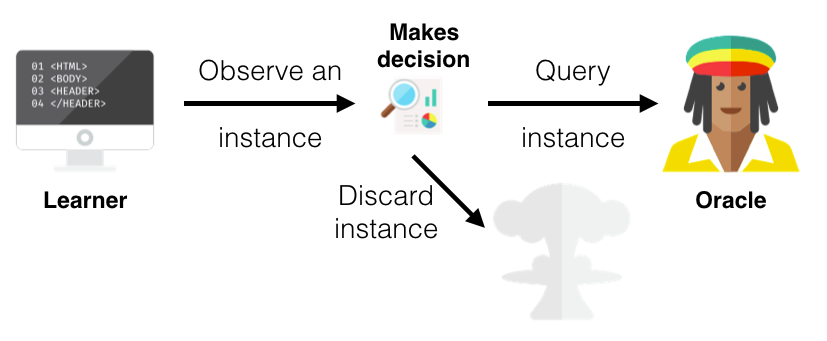
\includegraphics[scale=0.4]{images/stream_based}
	\caption{Stream-based selective sampling. Image from \cite{active_learning_datacamp}.}
	\label{stream_based}
\end{figure}\\
Fig \ref{stream_based} shows the workflow of membership query synthesis.The decision on querying the instance is decided by various query strategies that will be discussed in the upcoming section. \cite{Settles2010}\cite{active_learning_datacamp}
\subsection{Pool-Based Sampling}
The pool-based labeling setting consists of two pools of data which include a large set of unlabeled data and a small set of labeled ones. The instances are queried based on the usefulness to evaluate the other instances in the unlabeled pool.
\begin{figure}[h!]
	\centering
	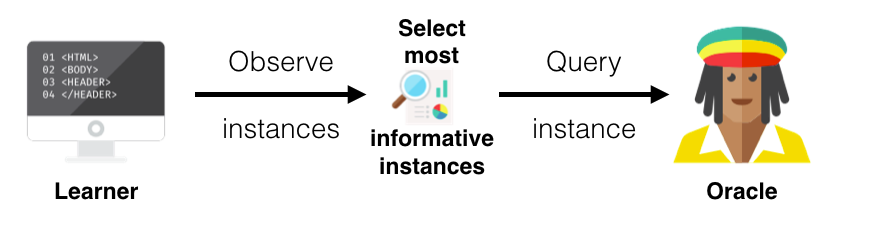
\includegraphics[scale=0.4]{images/pool_based}
	\caption{Pool-based selective sampling. Image from \cite{active_learning_datacamp}.}
	\label{pool_based}
\end{figure}\\

Fig \ref{pool_based} shows the workflow of membership query synthesis. This is different from the previous one where the data is queried from the stream of data coming whereas here the data is selected from the entire data pool based on its usefulness. \cite{Settles2010}\cite{active_learning_datacamp}
\section{Query strategy frameworks}
Passive learning approach has a large amount of labeled data which are sampled from an underlying distribution is used to train a model. Then the trained model is used for prediction. But in active learning, the learner query the most informative instance or the best instance which is the main difference between active and passive learning. There are various strategies to select the most informative query which are discussed below. \cite{Settles2010}

\subsection{Uncertainty Sampling}

Uncertainty sampling is a straightforward yet powerful active learning query strategy. In uncertainty sampling, the active learner query the data for which the prediction probability is very uncertain to classify into a  particular class. The three types of uncertainty sampling are discussed below.
   
\subsubsection{Least confident uncertainty sampling}

Least confident uncertainty sampling queries the instance for which the learner is not confident about its prediction. The instance that has to be queried using the least confident uncertainty sampling is found using the following equation given by \cite{lewis1994heterogeneous}. 

\begin{equation} 
x^{*}_{LC} = \operatorname*{argmax}_x  1 - P_{\theta}(\hat{y}|x) 
\end{equation}
Here,  $ P_{\theta}(\hat{y}|x) $ is the prediction probability of an instance belonging to a most likely class. This helps in finding the least confident instance for which the prediction probability for a particular class is high.
\begin{table}[htb!]
	\centering
\begin{tabular}{|c|c|c|c|}
	\hline
	\textbf{Instances} & \textbf{Class A} & \textbf{Class B} & \textbf{Class C} \\ \hline
	\textbf{I}         & 0.1              & 0.8              & 0.2              \\ \hline
	\textbf{II}        & 0.35             & 0.15             & 0.50             \\ \hline
	\textbf{III}       & 0.3              & 0.3              & 0.4              \\ \hline
\end{tabular}
	\caption{Prediction probabilty of three instances with respect to three classes}
	\label{least_confident}
\end{table}

For example, table \ref{least_confident} shows the prediction probability of the three instances from which one needs to be queried to the user for its label.From the table \ref{least_confident}, the uncertainties of the three data points are  0.2, 0.5 and 0.6 respectively. It is clear that the third instance has more uncertainty than the other two. Hence the third instance will be queried to the user by the active learner. \cite{Settles2010} \cite{modal_disagree}


\subsubsection{Margin uncertainty sampling}
Margin uncertainty sampling chooses instance considering the prediction probability of both the first and second likely class for which the instance belongs. This is in contrast to the least confident uncertainty sampling where it considers only the class for which the instance has maximum prediction probability. Scheffer et al.\cite{scheffer2001active}, computes the margin uncertainty of the instances using,
\begin{equation} 
 x^{*}_{M} = \operatorname*{argmin}_x P_{\theta}(\hat{y_{1}}|x) - P_{\theta}(\hat{y_{2}}|x)
 \end{equation} 

where, $P_{\theta}(\hat{y_{1}}|x)$ and $P_{\theta}(\hat{y_{2}}|x)$ were the prediction probability of the first and second likely class of a particular instance respectively. The instance for which the margin uncertainty is minimum is queried.

For example, let Table \ref{least_confident} shows the prediction probability of the three instances from which one need to be queried to the user for its label using margin uncertainty sampling. Margin uncertainty of first, second and third instance computed using the above equation are 0.6,0.15 and 0.1. Clearly, the third instance has less margin uncertainty which will be queried next.\cite{Settles2010} \cite{modal_disagree}

\subsubsection{Entropy uncertainty sampling} 
  
Entropy uncertainty sampling helps in overcoming the deficit of margin uncertainty sampling in cases where the number of classes is more. This is because margin uncertainty sampling considers only the first and the second most probable class.Entropy can be found using the below equation given by \cite{shannon1948mathematical}. 

\begin{equation} 
 x^{*}_{H} =   \operatorname*{argmax}_x - \sum_{i} ~ P_{\theta}(y_{i}|x) ~ log( ~ P_{\theta}(y_{i}|x)) 
 \end{equation} 
where $P_{\theta}(y_{i}|x)$ is prediction probability of instance x belonging to $i^{th}$ class. The instance for which the class probabilities closely represent a uniform distribution has more chance of having a higher entropy and being queried by the learner. \cite{Settles2010}
	
\subsection{Query-By-Committee}
Query-based committee algorithm has a committee which has a bunch of models. These models are trained on the available labeled data. Every model has its hypothesis. The central idea here is to select the instance in which there is more disagreement on the predictions among the models in the committee. This is done to bind the version space(all available set of hypotheses that are consistent with the labeled data). Query-based committee algorithm achieves this by selecting the instances in the disputed region. \cite{Settles2010} 

The disagreement among the models in the committee is measured mainly using the following three methods \cite{Settles2010}.

\subsubsection{Vote Entropy}

Vote entropy was proposed by \cite{dagan1995committee}. The vote entropy of each instance is found by using the below formula: 
\begin{equation} 
x^{*}_{VE} = \operatorname*{argmin}_x \sum_{i} \frac{V(y_i)}{C} log\frac{V(y_i)}{C}
\end{equation} 
in which 'i' refers to classes, '$V(y_i)$' refers to the count of votes that particular class achieves, and 'C' refers to the  number of models in the committee. The instance having the highest vote entropy value is queried \cite{dagan1995committee} \cite{Settles2010}.
This can be explained with an example based on \cite{modal_disagree}.Assume that there are three models, three classes(1,2 and 3) and five instances. Let the following table \ref{vote1} show the predicted label by each model. \\
\begin{table}[h!]
\centering
	\begin{tabular}{|c|c|c|c|}
		\hline
		\textbf{Instances} & \textbf{Model 1} & \textbf{Model 2} & \textbf{Model 3} \\ \hline
		\textbf{I}         & 1                & 1                & 1                \\ \hline
		\textbf{II}        & 2                & 2                & 1                \\ \hline
		\textbf{III}       & 3                & 1                & 1                \\ \hline
		\textbf{IV}        & 1                & 2                & 3                \\ \hline
		\textbf{V}         & 2                & 2                & 1                \\ \hline
	\end{tabular}
\caption{Predicted labels by the three models.}
\label{vote1}
\end{table}
Now the task is to select the instance with high vote entropy.  To find the vote entropy, probability distributions of each class have to be calculated first.  For the first instance, all the models predict 1. Hence the distribution for Class 1 is 1 and 0 for other classes. In the second instance, class 2 is selected twice. Therefore the distribution for Class 2 is 0.6667 (2/3) and for Class 1 is 0.3333(1/3). Similarly, the probability distribution for every class in other instances is found. The table \ref{vote2} shows the probability distribution of each class.
\begin{table}[h!]
	\centering
	\begin{tabular}{|c|c|c|c|}
		\hline
		\textbf{Instances} & \textbf{Class 1} & \textbf{Class 2} & \textbf{Class 3} \\ \hline
		\textbf{I}         & 1                & 0                & 0                \\ \hline
		\textbf{II}        & 0.3333           & 0.6667           & 0                \\ \hline
		\textbf{III}       & 0.6667           & 0                & 0.3333           \\ \hline
		\textbf{IV}        & 0.3333           & 0.3333           & 0.3333           \\ \hline
		\textbf{V}         & 0.3333           & 0.6667           & 0                \\ \hline
	\end{tabular}
\caption{Probability distribution on each class.}
\label{vote2}
\end{table}

Then the entropy for each instances is found and are displayed in table \ref{vote3}. 

\begin{table}[h!]
	\centering
	\begin{tabular}{|c|c|}
		\hline
		\textbf{Instances} & \textbf{Entropy} \\ \hline
		\textbf{I}         & 0                \\ \hline
		\textbf{II}        & 0.6365           \\ \hline
		\textbf{III}       & 0.6365           \\ \hline
		\textbf{IV}        & 1.0986           \\ \hline
		\textbf{V}         & 0.6365           \\ \hline
	\end{tabular}
	\caption{Entropy value for each instances.}
	\label{vote3}
\end{table}

From the table \ref{vote3}, it is very clear that the fourth instance has more vote entropy value. Hence the fourth instance will be queried. \cite{Settles2010}

\subsubsection{Consensus entropy}

Consensus entropy differs from the previous method by calculating the entropy values based on the consensus probabilities. The consensus entropy is calculated based on \cite{Settles2010} as, 
\begin{equation} 
P_c(y_i|x) = \frac{1}{C} \sum_{c=1}^{C} P_{\theta^(c)}(y_i|x)
\end{equation}  
where ‘C’ refers to the set of models in the committee, ‘x’ is the instance and $y_i$ is the predicted class. The above consensus probability is found by computing the mean of the class probabilities of each model in every instance.This can be explained with an example which is based on \cite{modal_disagree}.
Assume that there are four models, three classes(1,2 and 3) and five instances. The table \ref{con1} shows the class probabilities by every model in first instance.
\begin{table}[h!]
	\centering
	\begin{tabular}{|c|c|c|c|}
		\hline
		\textbf{Model}   & \textbf{Class 1} & \textbf{Class 2} & \textbf{Class 3} \\ \hline
		\textbf{Model 1} & 0.6              & 0.2              & 0.2              \\ \hline
		\textbf{Model 2} & 0.5              & 0.3              & 0.2              \\ \hline
		\textbf{Model 3} & 0.55             & 0.35             & 0.1              \\ \hline
		\textbf{Model 4} & 0.1              & 0.5              & 0.4              \\ \hline
	\end{tabular}
	\caption{Class probabilities by every model in first instance.}
	\label{con1}
\end{table}
Table \ref{con2} shows the calculated consensus probability. Then the entropy value for instance will be 1.06.
\begin{table}[h!]
	\centering
	\begin{tabular}{|c|c|c|}
		\hline
		\textbf{Class 1} & \textbf{Class 2} & \textbf{Class 3} \\ \hline
		0.44             & 0.34             & 0.22             \\ \hline
	\end{tabular}
	\caption{Consensus probability for each class of the first instance.}
	\label{con2}
\end{table}
Similarly the table \ref{con3} shows the class probabilities by every model in second instance. 
\begin{table}[h!]
	\centering
	\begin{tabular}{|c|c|c|c|}
		\hline
		\textbf{Model}   & \textbf{Class 1} & \textbf{Class 2} & \textbf{Class 3} \\ \hline
		\textbf{Model 1} & 0.3              & 0.2              & 0.5              \\ \hline
		\textbf{Model 2} & 0.3              & 0.5              & 0.2              \\ \hline
		\textbf{Model 3} & 0.35             & 0.15             & 0.5              \\ \hline
		\textbf{Model 4} & 0.2              & 0.3              & 0.5              \\ \hline
	\end{tabular}
	\caption{Class probabilities by every model in second instance.}
	\label{con3}
\end{table}
Table \ref{con4} shows the calculated consensus probability. Then the entropy value for instance will be 1.08.
\begin{table}[h!]
	\centering
	\begin{tabular}{|c|c|c|}
		\hline
		\textbf{Class 1} & \textbf{Class 2} & \textbf{Class 3} \\ \hline
		0.29             & 0.29             & 0.42             \\ \hline
	\end{tabular}
	\caption{Consensus probability for each class of the second instance.}
	\label{con4}
\end{table} 
Here the second instance is selected since it has more consensus value.	\cite{Settles2010}

\subsubsection{Max disagreement}
Max disagreement method was proposed by \cite{mccallumzy1998employing} based on KL divergence. KL divergence is used to measure the difference between the probability distributions \cite{kullback1951information}. The below equation for each instance helps in determining the KL divergence of each model to the consensus probability distribution according to \cite{kullback1951information}. 
\begin{equation} 
x^*_{KL} = \operatorname*{argmax}_x \frac{1}{C} \sum_{c=1}^{C} D (P_{\theta^(c)}|P_C), 
\end{equation} where 
\begin{equation}  D(P_{\theta^(c)}|P_C) = \sum_{i} P_{\theta^(c)}(\frac{y_i}{x}) log \frac{P_{\theta^(c)}(\frac{y_i}{x})}{P_{C}(\frac{y_i}{x})}  
\end{equation} 
Here $\theta^C$ denotes the parameters learned by models in the committee and  $P_c(y_i|x) = \frac{1}{C} \sum_{c=1}^{C} P_{\theta^(c)}(y_i|x)$ denotes the consensus probability for $y_i$ to be the right class. The instance having the high KL divergence value is queried. \cite{Settles2010}

\subsection{Expected Model Change}
Expected model change query strategy uses an approach called as “expected
gradient length” (EGL) which was proposed by \cite{settles2008multiple}.This approach can be used wherever the model is trained based on gradient descent. This type of query strategy chooses the instance which after labeling through querying can increase the gradient length. Gradient length refers to the vector that is used to update the parameters. The expected length is calculated using the following equation based upon the model’s current belief according to \cite{Settles2010}.

\begin{equation}  
x^*_{EGL} = \operatorname*{argmax}_x \sum_{i} P_{\theta}(\frac{y_i}{x})||\nabla l_{\theta}(L \cup <x,y_i>)||
\end{equation} 
where $\nabla l_{\theta}(L \cup <x,y_i>)$  refers to the gradient vector that been found by including the queried instance 'x' with the class '$y_i$' to the trained labeled data 'L'. \cite{Settles2010}

\subsection{Expected Error Reduction}
Expected Error Reduction query strategy in contrast to the previous query strategy(Expected model change query strategy) query the instance for which after labeling reduces the generalization error.  In this approach, the forthcoming error of the model is estimated based on the current belief and the instance which reduces the error more than others is queried.  The expected error change for all class possibility is estimated based on the model learned so far, since the true class for the queried label is unavailable during the estimation of the future error. The expected 0/1 loss is found using the below formula according to \cite{Settles2010}.
\begin{equation}  
x^*_{0/1} = \operatorname*{argmin}_x \sum_{i} P_{\theta}(\frac{y_i}{x})(\sum_{u=1}^{U} 1 - P_{\theta^{+<x,y_i>}}(\hat{y}|x^{(u)}))
\end{equation} 
where U refers to the set of instances on the unseen pool and $P_{\theta^{+<x,y_i>}}$ refers to the estimated probability of the instance based on the model trained after adding $<x,y_i>$ in the trained labeled dataset. The instance which minimizes the expected 0/1 loss is queried next. Instead of the expected 0/1 loss, the expected log loss can also be found and can be used in the selection of instance that can be queried. Likewise this method is not only constrained to minimization of the loss but also can be extended  to other  evaluation metrics such as maximizing precision, recall, f1 score etc., The computation cost for the expected error reduction is very high because it retrains the model for all the unseen instances to find the instance to be queried. Also it retrains the model after the query is labeled.  O(LUG) is the time complexity where L is the number of trained labeled dataset available so far, U is the number of unseen data in the pool, and G is the number of computation required to find the gradients. \cite{Settles2010}

\subsection{Variance Reduction}
Variance reduction helps in overcoming the shortcoming of the expected error reduction query strategy where the computation cost is very high. This is achieved by decomposing the expected error based on the approach given by \cite{geman1992neural} as 
\begin{equation} 
E_T[(\hat{y} - y)^2|x] = E[(y - E[y|x])^2] + (E_L[\hat{y}] - E[y|x])^2 + E_L [(\hat{y} - E_L[\hat{y}])^2]
\end{equation} 
where $E_L$  refers to the expectation on the already available labeled set, E refers to the expectation on the probability of the true label given  an instance and $E_T$ combine both the previous expectation, $E[(y - E[y|x])^2] $is the variance which does not depend in the training data, $(E_L[\hat{y}] - E[y|x])^2$ is the bias and does not affect the generalization error. Hence only $E_L [(\hat{y} - E_L[\hat{y}])^2] $ can affect the generalisation error of the model as this is the variance of the model. Here the model’s variance refers to the models mean squared loss.The variance reduction query strategy can be implemented by finding the value of $x^*_{VR}$ for all the unseen instances using the below formula and the instance which reduces the variance is queried to the user. 
\begin{equation}  
x^*_{VR} =  \operatorname*{argmin}_x {<\widetilde{\sigma}^2_y >}^{+x} 
\end{equation} 
where ${<\widetilde{\sigma}^2_y >}^{+x}$ is the estimated mean output variance. The instance which reduces this variance also reduces the generalization error. \cite{Settles2010} \cite{chaloner1995bayesian} \cite{cohn1995active}

\subsection{Density-Weighted Methods}
Density weighted method while querying not only considers the data in the uncertain region but also the input space’s dense region. This is done to avoid querying the instances that are outliers. Uncertainty based sampling and Query by committee methods suffers from this problem. Sometimes they query the outliers. This can be illustrated from the figure \ref{weight} shown below.

\begin{figure}[h!]
	\centering
	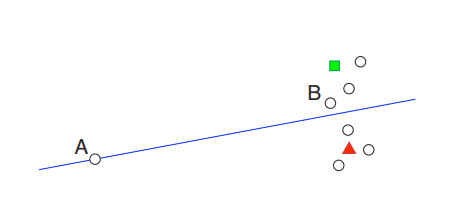
\includegraphics[scale=0.7]{images/density}
	\caption{Outlier point A will get queried instead of point B since it lies very close to the uncertain region. Image from \cite{Settles2010}}
	\label{weight}
\end{figure}


In the figure \ref{weight}, the triangle and square represent the data for which the classes are known already. The circle represents the data in the dense pool. Now the uncertainty based sampling will query the data point A since it lies close to the margin. However, point B is the most useful query in this situation.  This problem can be avoided if the instances are queried in the dense region.

Instance are queried based on the below formula given by \cite{settles2008analysis},

\begin{equation}  
x^*_{ID} =  \operatorname*{argmax}_x \phi_{A}(x) * (\frac{1}{U} \sum_{u=1}^{U} sim (x,x^{(u)})) ^\beta 
\end{equation} 
where $\phi_{A}(x)$ refers to the informativeness based on any other query strategy and $(\frac{1}{U} \sum_{u=1}^{U} sim (x,x^{(u)})) ^\beta$  refers to the weight of the informativeness. Sim here refers to the similarity measures like cosine distance, Euclidean distance or KL divergence.The computation cost increases quadratically with the number of unseen instances. This can be optimized by having a look-up table or precomputed data. \cite{settles2008analysis} \cite{Settles2010}


 